\chapter{Incorporating interactions}
\label{ch:chapter_3}

\begin{abstract}
In this chapter, I include interactions into the non-equilibrium Green's Function formalism. In particular, I focus on capacitive interactions (e.g. Coulomb interaction) as these are the primary investigation of this thesis. I formulate a many\hyp{}body Green's function that incorporates capacitive interaction. I also find a self-consistency equation for the non-equilibrium density matrix. Additionally, some attention is given to electron-phonon interactions, leading to a very similar many-body Green's function that incorporates these interactions.
\end{abstract}

%% Start the actual chapter on a new page.
\newpage
\section{Introduction}
This chapter is mostly self-contained; it is about two new derivations. Note that the capacitive interaction derivation was first performed by Dr. Jos Seldenthuis, but not previously published.

We consider a rather general model system, that consists of a diagonal Hamiltonian representing the molecular orbits, a tunnelling term and  two-particle interaction, which is approximated as capacitive interaction. For this generalised system we can find a closed expression which includes the capacitive interaction.

We will see that the result is conceptually simple, merely an expectation value of the Green's Function of every many-body state. It turns out that this conceptual picture is also a valid derivation of the many-body Green's function in closed form.

We then consider a model system that is also coupled to a single vibrational mode. The only term that does not commute with the electron annihilation operator is that of an electronic transition in which a phonon is absorbed or emitted, corresponding to the phononic annihilation and creation operators.

Nevertheless, this is the point where people have often turned away from that derivation because it seems like that phononic self\hyp{}energy term is not captured easily in the NEGF formalism. However, the methods used to find the capacitive interaction are found to work for the phononic self-energy as well. The result is extremely elaborate because of a expansion for arbitrary powers of the sum of non-commuting terms. 

The outline of this chapter is as follows. First, we discuss a generalised number operator for many-body states in section~\ref{sec:gno}. Next, I calculate the capacitive self-energy in section~\ref{sec:capacitive}. The result is defined as a matrix-inverse which seems ill-defined, so I develop the expression in section~\ref{sec:mbgfno}. A matrix equation defining the non-equilibrium density of states and a self-consistent scheme to solve it are given in section~\ref{sec:densitymatrix}.The expression for current is given in section~\ref{sec:calcprop}. Finally, we discuss the novel interaction treatment in section~\ref{sec:discussioncapacitive}.

Then we briefly consider vibrational interactions and include these in a similar manner as the capacitive interactions in section~\ref{sec:phononic}. We discuss the result and a preliminary figure in section~\ref{sec:phononicdiscussion}. However, we do not continue with vibrational modes because of time constraints.
\section{Generalised Number Operator}
\label{sec:gno}


I will use the convention that \emph{latin} subscripts indicate molecular orbits and \emph{greek} subscripts indicate many-body states\footnote{This convention is used because molecular orbits are more common throughout this work.}. Each many-body state is a set of indices corresponding to occupied single-particle states. I define the following:
\begin{align*}
\Psi_\kappa (t) &\equiv \sum_{ \left\{\kappa\right\}} C_\kappa(t) a_\kappa^\dagger \ket{0}, \\
a^\dagger_\kappa &\equiv \prod_{ i \in \left\{\kappa\right\}} a_i^\dagger, \\
\rho_{\kappa,\kappa^\prime} & \equiv C_{\kappa'}^\star (t) C_\kappa (t),
\\
\widehat{\rho}_{\kappa\kappa^\prime}(t) &\equiv \rho_{\kappa,\kappa^\prime} (t) a_{\kappa}^\dagger \ket{0}\bra{0}a_{\kappa^\prime}.
\end{align*}

Now, we want to look at the `generalised' number operator, defined in a manner similar to ordinary number operators: 
\begin{align}
n_{\kappa\kappa^\prime} &\equiv a^\dagger_\kappa a_\kappa \label{eq:gennum}
\end{align}
While its purpose is not yet clear, it is an interesting operator to look at in its own right.Its expectation value is:
\begin{align*}
n_{\kappa\kappa^\prime} (t) &= \braket{\Psi (t) \left| \widehat{n}_{\kappa\kappa^\prime}\right|\Psi (t)} \\
&=\sum_{\lambda\lambda^\prime} \braket{0\left| C_\lambda^\star (t) C_{\lambda^\prime} (t) a_\lambda a_\kappa^\dagger a_{\kappa^\prime} a_{\lambda^\prime}^\dagger \right|0}
\\
&= \sum_{\lambda\lambda^\prime} \rho_{\lambda\lambda^\prime} \braket{0\left| \prod_{p \in \lambda\setminus{\kappa}} a_p a_\kappa a_\kappa^\dagger a_{\kappa^\prime} a_{\kappa^\prime}^\dagger \prod_{q \in \lambda^\prime\setminus{\kappa^\prime}}a_q^\dagger \right|0}
\\
&= \sum_{\lambda\lambda^\prime} \rho_{\lambda\lambda^\prime} \prod_{p \in \lambda\setminus{\kappa} \wedge q \in \lambda^\prime\setminus{\kappa^\prime}} \tilde{\delta}_{pq}
\\
&=  \sum_{\lambda\lambda^\prime} \rho_{\lambda\lambda^\prime},
\end{align*}with the following conditions:
\begin{itemize}
\item $\lambda\supseteq\kappa$. The story here is a bit confused, because $\kappa$ itself is some sort of set. In principle, it means that the orbital occupation in $\kappa$ is the minimum for a possible $\lambda$. So if $\kappa$ specifies orbitals $i$ and $i^\prime$ are occupied, then for all $\lambda$ the orbitals $i$ and $i^\prime$ are occupied. This allows for the expansion that includes the subscripts $p$ and $q$.
\item The set differences $\lambda\setminus{\kappa}$ and $\lambda^\prime\setminus{\kappa^\prime}$ must be equal, otherwise the creation and annihilation operators do not cancel out. 
\item $\tilde{\delta}$ is a very imprecise term, which reduces to zero except when the states $p$ and $q$ in the product are taken from one and the same set, in which case it yields unity.
\end{itemize}

The effect of the generalised number operator $n_\kappa$ on some arbitrary many-body state $\kappa'$ is:
\begin{align}
\bra{\kappa'} n_\kappa \ket{\kappa'} &= \begin{cases} 1 &\quad \kappa'\supseteq\kappa \\
0 & \quad \text{otherwise} \end{cases}
\label{eq:generalisednumberoperator}\\
&\equiv \Delta^{\kappa}_{\kappa'}\nonumber
\end{align}
where $\Delta^{\kappa}_{\kappa'}$ is a convenient short hand.

\section{Capacitive Interactions} 
\label{sec:capacitive}
In section~\ref{sec:eommethod} I have already discussed the molecule and the leads. I will now separate the tunnelling between levels from the molecule Hamiltonian. The interaction between electron states is between two electrons. While there might be perhaps three and more particle interactions, we do not consider them at this time. We are looking for Coulomb interactions which are of the two-particle type.

The device interaction Hamiltonian has the following form:
\begin{align*}
H^\prime_D &= \frac{1}{2} \sum_{ijkl} W_{ijkl} d^\dagger_i d_j d^\dagger_k d_l \\
&\approx \frac{1}{2} \sum_{ij} U_{ij} n_i n_j,
\end{align*} where the approximation effectively assumes that the capacitive interactions do not mix the eigenstates of the unperturbed Hamiltonian. In other words, removing an electron is assumed only to change the energy of the other electrons but not their spatial distribution. Since each electron feels only the combined density of all other electrons, removal and addition of a single electron from a large molecule or quantum dot is only a small perturbation. Moreover, we are generally interested in HOMO and LUMO transport, which for conjugated molecules are orbitals that are delocalised over the entire molecule.

The commutator of the annihilation operator with the capacitive interaction term is easily found:
\begin{align*}
\left[ d_l, H^\prime_D\right] &= \sum_{j} \frac{1}{2} \left( U_{lj} + U_{jl}\right) n_j d_l + U_{ll} d_l.
\end{align*}
The last term is capacitive self-interaction, which is unphysical and therefore zero. Likewise,the symmetry of the Hamiltonian specifies that $U_{ij} = U_{ji}$ and that $U_{ij} \in \Re$. Thus, we find that:
\begin{align*}
\left[ d_i, H^\prime_D\right] &=  \sum_{j}U_{ij} n_j d_i \\
&= \sum_j U^j_{ij} n_j d_i,
\end{align*}
where I have defined $U^k_{ij} = U_{ik} \delta_{ij}$ to simplify future expressions. We then turn to the Fourier-transformed full time derivative of the Green's Function:
\begin{align*}
\epsilon G_{ij}^\pm &= \delta_{ij} + \epsilon_i G_{ij}^\pm + \sum_k \tau_{ik} G_{kj}^\pm + \sum_k U^k_{ik} n_k G_{ij}^\pm,
\end{align*}
where comparison with the Dyson equation (equation~\ref{eq:dyson}) shows us that the capacitive self-energy is:
\begin{align}
\Sigma^{c} &= \sum_k U^k n_k
\label{eq:selfenergycapacitive}
\end{align}While I can now express the Green's function as $G^\pm = \left[ \epsilon - \epsilon_i - \tau - \Sigma^c \pm \imath 0^+\right]^{-1}$, the capacitive self-energy is still an operator while the other contributions are matrices. Additionally, I am taking the inverse of a series of number operators. 

\section{The Many-Body Green's Function and Number Operators}
\label{sec:mbgfno}
The matrix inverse in the previous section might seem ill-defined, because we took the inverse of a series of number operators. However, we can get a well-defined expression by Taylor expanding the matrix inverse in $B$, e.g.:
\begin{align}
\left[ A^{-1} - B\right]^{-1} &= A + ABA + ABABA + \ldots
\label{eq:inversionexpansion}
\end{align}

If you recall, the common single-particle retarded (advanced) Green's functions are $G = \left[ g^{-1} \pm \Sigma \right]^{-1}$, which would be expanded as $G = g + g\Sigma g + g\Sigma g\Sigma g + \ldots$ - which is the expansion in arbitrary order we used intuitively to arrive at the Dyson equation (equation~\ref{eq:dyson}). Let's look explicitly at the result for two-particle Green's Function in the WBL:
\begin{align*}
G^\pm  &= \left[ A^{-1} - B_1 n_1 - B_2 n_2 \right]^{-1},
\end{align*}
where 
\begin{align*}
A &= \begin{bmatrix} \epsilon - \epsilon_1 - \Sigma^\pm & \tau \\ 
\tau & \epsilon - \epsilon_2 - \Sigma^\pm \end{bmatrix},\\
B_1 &= \begin{bmatrix} 0 & 0 \\ 0 & U \end{bmatrix},\\
B_2 &= \begin{bmatrix} U & 0 \\ 0 & 0 \end{bmatrix}
\end{align*}

I apply the Taylor expansion (equation~\ref{eq:inversionexpansion}) and group the number operators, so that I obtain:
\begin{align*}
G^+ &= A + A\left[B_1 n_1 + B_2 n_2\right]A + A\left[B_1 n_1 + B_2 n_2\right]  A\left[B_1 n_1 + B_2 n_2\right]  A + \ldots \\
&= (1-n_1)(1-n_2) A + n_1 (1-n_2)\left[A + AB_1 A + AB_1AB_1A + \ldots \right] + \\
&\quad (1-n_1)n_2 \left[ A + AB_2A + AB_2AB_2A + \ldots \right] +\\
&\quad n_1 n_2 \left[ A + A\left[B_1 + B_2\right]A+ A\left[B_1 + B_2\right]A\left[B_1 + B_2\right]A + \ldots\right] \\
&= (1-n_1)(1-n_2) A + n_1 (1-n_2) \left[ A^{-1} - B_1\right]^{-1} + (1-n_1) n_2 \left[ A^{-1} - B_2\right]^{-1} +\\&\quad n_1 n_2 \left[A^{-1} - B_1 - B_2 \right]^{-1}
\end{align*}

The idea is to group terms with the same combination of occupation number operators while taking into account the fact that $n_i = n_i n_i$ and that $n_i = (1-n_j)n_i + n_j n_i$  for fermions. We only show the extension to more particles, for which the general result is\footnote{I will use $\mathscr{E}$ for the variable, the rest are matrices}:
\begin{align}
G &= \left[ \mathscr{E} - \epsilon - \tau -\Sigma^{d\pm} - \Sigma^\pm \right]^{-1} \nonumber\\
&= \sum_\kappa \left( \prod_{i\in\kappa} \prod_{j\notin\kappa} n_i (1-n_j) \right) \left[ \mathscr{E} - \epsilon -\tau - \sum{i \in \kappa}U^i - \Sigma^\pm \right]^{-1} \nonumber\\
&= \sum_\kappa P_{\kappa\kappa} \left[ \mathscr{E} - \epsilon - \tau - \sum_{i\in\kappa} U^i - \Sigma^\pm \right]^{-1} \label{eq:grouping}
\end{align}
where $k$ sums over all possible combinations of occupation number operators or equivalently all many-body states. Note that $P_{kk}$ is the diagonal of the probability operator, so that its expectation value is the diagonal of the reduced density matrix of the device. I want to discuss transport through a specific many-body state $\kappa$. Therefore, I define the many-body Green's Function as:
\begin{align}
\mathscr{G}^{\kappa\pm}_{ij} (t,t') &= \mp \frac{\imath}{\hbar} \theta(\pm(t-t'))\left\{ n_\kappa d_i(t), d_j^\dagger (t')\right\},
\label{eq:mbgfdef}
\end{align}
where we have included the generalised number operator (equation~\ref{eq:gennum}). We can find the commutator of $n_i$ with the lead-molecule Hamiltonian $H'$ and the tunnelling Hamiltonian $H_\tau$, which is nonzero and therefore prevents us from obtaining a closed expression for the many-body Green's function in matrix form. We therefore assume $\left[ n_i, H' + H_\tau \right]=0$, which is equivalent to cutting off tunnel couplings after first order. Then, the many-body Green's function is:
\begin{align}
\mathscr{G}^{\kappa\pm} &= \left[ \epsilon - \epsilon_i - \tau - \Sigma^c - \Sigma^\pm\right]^{-1} n_\kappa,
\label{eq:mbgfmatrix}
\end{align}
where $\epsilon_i$ reflects the fact that I've taken $H_1$ to be diagonal with $\epsilon_i$ on the diagonal. I can then find the expectation value of the many-body Green's Function :
\begin{align}
\mathscr{G}^{\kappa\pm} &= \sum_{\lambda\lambda'} C_\lambda C^\star_{\lambda'} \braket{\lambda \left| \left[ \epsilon - \epsilon_i - \tau - \Sigma^c - \Sigma^\pm\right]^{-1} n_\kappa \right| \lambda'} \nonumber \\
&= \sum_{\lambda,\lambda'\supseteq\kappa} C_\lambda C^\star_{\lambda'} \braket{\lambda \left| \left[ \epsilon - \epsilon_i - \tau - \Sigma^c - \Sigma^\pm\right]^{-1} \right| \lambda'} \nonumber \\
&= \sum_{\lambda,\lambda'\supseteq\kappa}  C_\lambda C^\star_{\lambda'} \braket{\lambda|\lambda'}  \left[ \epsilon - \epsilon_i - \tau - \sum_{p \in \lambda'} U_{ip} - \Sigma^\pm\right]^{-1}
\\&= \sum_{\lambda\supseteq\kappa} P_{\lambda\lambda} G^{\lambda\pm},\label{eq:mbgfresult}
\end{align}
where 
\begin{align*}
G^{\lambda\pm} &= \left[\mathscr{E} - \mu^\lambda - \tau - \Sigma^\pm \right]^{-1},
\end{align*}
in which
\begin{align}
\mu^\lambda_{ij} &= \delta_{ij} \left( \epsilon_i + \sum_{p\in\lambda} U_{ip} \right) \label{eq:result},
\end{align} in which $H^\kappa = \mu^\kappa + \tau$ is recognised as the effective single-particle Hamiltonian of the system in the many-body state $\kappa$. This can be directly obtained from DFT calculations. This is a very useful fact, as some molecules are hard to capture otherwise, e.g. Ref.~\cite{frisenda}. In particular, \emph{many} DFT calculations together can give us (a good approximation of) the full shape of $H^\kappa$, leading to a more complete description of transport through the formulae derived above. In particular the formalism should be more accurate for excitations, and could potentially explain coulomb blockades. This is a useful result for molecules that aren't accurately described as a set of weakly coupled moieties.

\section{Calculating Properties}
\label{sec:calcprop}
A simpler derivation for the expectation value of the Green's Function is possible. We use the definition of equation~\ref{eq:mbgfmatrix}. The expectation value makes good use of the properties of the generalised number operator (equation~\ref{eq:generalisednumberoperator}). First, recall the expectation value of the many-body wavefunction $\ket{\Psi}$:
\begin{align*}
\ket{\Psi} &= \sum_\lambda C_\lambda \ket{\lambda}.
\end{align*}
It is then relatively simple to evaluate:
\begin{align*}
\braket{\lambda^\prime \left| \mathscr{G}^\kappa \right| \lambda } &= 
\braket{\lambda^\prime \left|  G n_\kappa \right| \lambda } \\
&= \braket{\lambda^\prime \left| G \Delta^\lambda_\kappa \right| \lambda },
\end{align*} where the operators are separable with respect to the expectation value by virtue of the general result of Taylor expanding and grouping the number operators (equation~\ref{eq:grouping}).
Because the retarded (advanced) Green's function only had a remaining capacitive self-energy operator (equation~\ref{eq:selfenergycapacitive}), which is a diagonal operator, I can Taylor-expand the Green's function as we did before (equation~\ref{eq:inversionexpansion}). Since $\bra{\lambda'}n_i \ket{\lambda}=\Delta^\lambda_i\braket{\lambda'|\lambda}$\footnote{Yes, $i \in \lambda$ is equivalent to $\lambda\supseteq i$!}, without changing the state, we can just write down the 'number', as opposed to operator,  $G^\lambda$! 
\begin{align*}
&= \braket{\lambda^\prime \left| \left[ A + ABA + ABABA \right] \Delta^\lambda_\kappa \right| \lambda } \\
&=  G^\lambda \Delta^\lambda_\kappa \braket{\lambda^\prime | \lambda }\\
&=  G^\lambda \Delta^\lambda_\kappa \delta^\lambda_{\lambda^\prime}.
\end{align*}
Therefore, to evaluate the many-body Green's function, I simply take its expectation value:
\begin{align*}
\braket{ \mathscr{G}^{\kappa\pm}} &= \sum_{\lambda,\lambda^\prime}C_{\lambda^\prime}C_\lambda^\star \braket{\lambda^\prime \left| \mathscr{G}^{\kappa\pm} \right| \lambda } \\
&= \sum_{\lambda,\lambda^\prime} C_{\lambda^\prime}C_\lambda^\star  G^{\lambda\pm} \Delta^\lambda_\kappa \delta^\lambda_{\lambda^\prime}\\
&= \sum_{\lambda \supseteq \kappa} \rho_{\lambda\lambda}(t) G^{\lambda\pm} .
\end{align*}
This derivation is apparently less complicated. It makes use of the same expansion as the earlier derivation, but by immediately looking for the expectation value of the Green's function rather than the intermediary operator form, it becomes a simpler derivation. Starting from the Keldysh equation (equation~\ref{eq:keldysh}), we can derive the many-body lesser Green's function from the advanced and retarded ones:
\begin{align*}
    \mathscr{G}^{\kappa<} &= \mathscr{G}^{\kappa+} \Sigma^< \mathscr{G}^{\kappa-} \\
    &= \sum_{\lambda\supseteq\kappa, \lambda^\prime \supseteq\kappa}P_{\lambda'\lambda'} P_{\lambda\lambda} G^{\lambda+} \Sigma^< G^{\lambda^\prime-}.
\end{align*}
Making use of the fact that $P$ is diagonal and using the Keldysh equation for the Green's function, I find:
\begin{align}
    \mathscr{G}^{\kappa<} &= \sum_{\lambda\supseteq\kappa} P_{\lambda\lambda} G^{\lambda<} \label{eq:mblessergf},
\end{align} where I have used that $P_{\kappa\kappa} \ket{\kappa'}$ is $\ket{\kappa}$ if $\kappa'=\kappa$ and zero otherwise. The above shows that the expectation value of the many-body Green's Function (equation~\ref{eq:mbgfmatrix}) can immediately yield the correct expressions without grouping the occupation number operators.
The derivation of the current is straightforward. It can be motivated by looking at the expectation value,  $\braket{I}$. The current is a eigenvalue, in the sense that $ \widehat{I} \ket{\kappa} = I^\kappa \ket{\kappa}$. As a result, the expectation value will become a sum of diagonal density matrix elements times the current in that many-body state. The current in that many-body state is then rather trivially equation~\ref{eq:landauer} but with the many-body Green's function substituted, i.e. $G \rightarrow \mathscr{G}^{\kappa\pm}$.

Finally, we state the result for the current:
\begin{align*}
\widehat{I} &\equiv \sum_\kappa P_{\kappa\kappa} \braket{ \kappa \left|\widehat{I}\right|\kappa}=\sum_\kappa P_{\kappa\kappa} \widehat{I}^k,\\ 
I(t) &= \sum_\kappa \rho_{\kappa\kappa}(t) I^\kappa, \\
I^\kappa&\equiv \frac{e}{\hbar} \int^\infty_{-\infty} \frac{d\epsilon}{2\pi} \left[ f_L(\epsilon) - f_R (\epsilon) \right] T^\kappa (\epsilon),\\
T^\kappa(\epsilon) &\equiv \text{Tr}\left\{ \Gamma^L \mathscr{G}^{\kappa+} \Gamma^R \mathscr{G}^{\kappa-} \right\}.
\end{align*}



\section{Density Matrix}
\label{sec:densitymatrix}
Many quantum problems are concerned with finding the density matrix of the system, a problem that is only enhanced in non-equilibrium situations. This is even more troublesome when interaction is included. In this section I outline a convenient method for the calculation of the density matrix $\rho(t)$, more accurately its diagonal $P_\kappa$.

The starting point is the expectation value of a single-particle number operator $n_i$. This is the occupation probability of the single-particle state, not that of the many-body state where it is the singularly occupied state. It is related to the many-body occupation probabilities via:
\begin{align*}
\braket{n_i} &= \sum_{\kappa: i \in \kappa} P_\kappa,
\end{align*} where the sum is over those $\kappa$ in which $i$ is occupied. These equations are linear, and by defining $K$ they can be written in matrix form. I choose to write the matrix elements as $K_{i\beta}$ to emphasise that $i$ corresponds to a single-particle state while $\beta$ to a many-body state:
\begin{align*}
K_{i\beta} &\equiv \begin{cases} 1 & i \& \beta = i\\ 0 & \text{otherwise} \end{cases},
\end{align*} where $\&$ is the binary `and' operator. The matrix equation for expectation values of a single-particle number operators is then found to be:
\begin{align*}
\braket{n_i} &= \sum_{\beta} K_{i\beta} P_\beta, 
\end{align*}
so that the vector of single-particle number operators is obtained as:
\begin{align}
\braket{n} &= K P \label{eq:nkp}.
\end{align}

For instance, in a system with three single-particle states the explicit expression becomes \cite{seldenthuis}:
\begin{align*}
\begin{pmatrix} \braket{n_1} \\\braket{n_2} \\ \braket{n_3}\end{pmatrix} &= \begin{pmatrix} 0 & 1 & 0 & 1 & 0 & 1 & 0 & 1 \\ 0 & 0  &  1  & 1 & 0  &  0  &  1  &  1\\ 0 & 0 & 0 & 1 & 0 & 0 & 0 & 1\\\end{pmatrix} \begin{pmatrix} P_{\ket{000}} \\P_{\ket{001}} \\ P_{\ket{010}} \\ P_{\ket{011}} \\ P_{\ket{100}} \\ P_{\ket{101}} \\ P_{\ket{110}} \\ P_{\ket{111}} \end{pmatrix}.
\end{align*}

The expectation values of single-particle number operators can also be obtained from the  many-body lesser Green's Function at $t=t'$:
\begin{align*}
\braket{n_i} &= \sum_{\kappa: i \in \kappa} \braket{n_\kappa d_i^\dagger (t) d_i (t)} \\
&= \sum_{\kappa: i \in \kappa} \braket{\mathscr{G}^{\kappa<}_{ii}} \\
&= \sum_{\kappa: i \in \kappa} \sum_{\lambda \supseteq \kappa} P_\lambda \int^\infty_{-\infty} \frac{d\epsilon}{2\pi\imath} G^{\lambda<}_{ii} (\epsilon) \\
&= \sum_{\kappa: i \in \kappa} \sum_{\lambda \supseteq \kappa} P_\lambda \int^\infty_{-\infty} \frac{d\epsilon}{2\pi\imath} \left[ \sum_\alpha f_\alpha(\epsilon) G^{\lambda+}_{ii} (\epsilon) \Gamma^\alpha G^{\lambda-}_{ii} (\epsilon)\right] \\
&= W_{i,1} P_{\kappa_1} + W_{i, 2} P_{\kappa_2} + \ldots \\
&= \sum_\kappa W_{i\kappa} P_\kappa,
\end{align*} where the lesser self-energy is substituted from equation~\ref{eq:lesserself}. The matrix element $W_{i\beta}$ is defined as:
\begin{align*}
W_{i\beta} &= \sum_{\kappa: i \in \kappa} \Delta^\beta_\kappa \int^\infty_{-\infty} \frac{d\epsilon}{2\pi\imath} \left[ \sum_\alpha f_\alpha(\epsilon) G^{\lambda+}_{ii} (\epsilon) \Gamma^\alpha G^{\lambda-}_{ii} (\epsilon)\right],
\end{align*} where $\Delta^\beta_\kappa$ ensures only those $\kappa$ that are in the superset of $\beta$ are counted (equation~\ref{eq:generalisednumberoperator}). Thus I obtain a matrix equation for the vector of expectation values of single-particle number operators:
\begin{align}
\braket{n} &= WP. \label{eq:nwp}
\end{align}

Equations~\ref{eq:nkp} and~\ref{eq:nwp} are both exact, so consistency requires that:
\begin{align}
WP &= KP. \label{eq:selfconsistency}
\end{align}

Now, it is not guaranteed that the solution to this equation is unique or equivalently that the null-space of $W-K$ is one-dimensional. In practise, one would start from an equilibrium situation and take the ground state occupation probability as the initial guess, so that the non-equilibrium interactions can be turned on adiabatically. In this way, we can solve the system adiabatically to obtain the non-equilibrium ground state. This can be interpreted as a variation of the Gell-Mann and Low theorem \cite{gellmannlow, molinari}.

Since $W-K$ is a matrix with the amount of rows equal to the dimension of the Hamiltonian or equivalently the maximum number of electrons $N$. However, the number of columns is equal to the amount of many-body states $2^N$, so that the inverse of either $W$ or $K$ can't be found. A practical algorithm would start from an initial guess $P^0$, likely the (equilibrium) Boltzmann distribution. The next step is to calculate $WP^0$, which should equal $KP^1$. The next iteration $P^1$ is then found by a minimisation procedure. This self-consistent loop is repeated until it converges on the non-equilibrium steady state $P_\lambda$.



\section{Discussion of Capacitive Interactions}
\label{sec:discussioncapacitive}
It is of interest to consider how our approximation and the result (eq~\ref{eq:result}) compare to other results, for instance the BBGKY hierarchy (see Ref.~\cite{diventra}).

It is relatively simple to show that our results only treat a subset of the BBGKY hierarchy. If we start from a relatively simple Hamiltonian that includes two-body interaction:
\begin{align*}
H &= -\sum_i \frac{\hbar^2}{2m} \nabla_i^2 + \sum_{ij} w(r_i - r_j).
\end{align*}
The resulting Heisenberg equation for the field operator $\psi$ reads:
\begin{align*}
\imath\hbar\partial_t \psi(r, t) &= -\frac{\hbar^2}{2m} \nabla^2 \psi(r,t) + \int dr^\prime \: \left[ w(r-r^\prime) \psi^\dagger (r^\prime, t) \psi(r^\prime,t) \psi(r,t)\right].
\end{align*}

Note that the Feynman Diagrams of such an interaction are in principle unlimited; one can make many, many transitions and later re-absorb the sum of these transitions to transition back. We would then expect, similar to the non\hyp{}interacting contacts case, to simply expect a contribution to the self-energy directly obtained from comparison of the equation of motion method result with the Dyson equation.

From there, we can find the equation of motion for the single-particle time-ordered Green's function:
\begin{align*}
G(r,t;r^\prime,t^\prime) &= -\frac{\imath}{\hbar}\braket{T \left\{ \psi(r,t) \psi^\dagger(r^\prime,t^\prime)\right\}}, \\
\left(\imath\hbar\partial_{t_1} + \frac{\hbar^2}{2m}\nabla_i^2\right) G(r_1, t_1; r_1^\prime, t_1^\prime) &= \delta(r_1 - r_1^\prime) \delta(t_1 - t_1^\prime) \\&- \imath \int dr\left[w(r_1 - r) ) \psi^\dagger (r^\prime, t) \psi(r^\prime,t) \psi(r,t) \psi(r_1^\prime, t_1^\prime)^\dagger\right]
\end{align*}

If I now expand the field operators into particle operators, with $\phi_k$ representing a single-particle wave function:
\begin{align*}
\psi(r, t) &= \sum_k \braket{r|\phi_k} a_k,\\
\psi(r, t)^\dagger &= \sum_k \braket{\phi_k|r} a_k^\dagger,\\
\int dr\ldots &= \int dr \sum_{ijkl} W_{ijkl} a_i(t_1) a_j (t_1) a_k^\dagger(t_1^+) a_l^\dagger(t_1^\prime),
\end{align*} which is the interaction term I included in my general model. As a result, the capacitive approximation I used in section~\ref{sec:capacitive} to obtain the term $\frac{1}{2} \sum_{ij} U_{ij} n_i n_j$ regards only a subset of the BBGKY hierarchy, which is to be expected due to the presence of not only contacts but alsoo a many-body interaction that is usually hidden in the effective Hamiltonian calculated by DFT.

In a paper by Datta\cite{mura}, they outline that the rich spectrum of excitations is problematic to capture within any self-consistent field (SCF) theory. They illustrate this problem by elaborating on a spin-degenerate level that is specific example of the general model discussed above. They mostly use this as a motivation for turning to a Master Equation Approach.  It is pertinent because they specifically mention that the SCF approach misses the fact that subsequent spin addition/removal processes need not contribute equally to the overall current.

My derivation above explicitly incorporates the many-body character of the problem with capacitive interactions, and should therefore be capable of capturing such effects.

From my derivation and the discussion above, it seems that this extension to the formalism does include the relevant electron-electron interactions and should prove to be a method to calculate the Coulomb Blockade in a consistent manner within the non-equilibrium Green's Function formalism. Keep in mind that, in addition to cutting off tunnelling couplings after first order, I only regard a subset of the BBGKY hierarchy.



\section{Phonons}
\label{sec:phononic}

Vibrational modes are briefly considered here. Bosonic interactions are the inclusion of phonon or photon interaction with electronic transitions. For instance, one could consider photon emission where the transition from state $\ket{i}$ to $\ket{i'}$ is paired with the emission of a photon at energy $\hbar \omega$, called electroluminescence \cite{electroluminescence}. An interaction term of this sort would have the form $\hbar\omega b^\dagger d_{i'}^\dagger d_i$, where $b$, $b^\dagger$ are bosonic annihilation and creation operators.

I consider vibrational excitations of a single mode in weakly coupled single-molecule junctions using a generalisation of the above relation, which is in principle correct for phonons as well as photons. The generalisation is also known as a Fr\"ohlich interaction and the resulting Hamiltonian is known as the Fr\"ohlich Hamiltonian \cite{frohlich}. The Hamiltonian is given by adding the following terms to the device-Hamiltonian (including capacitive interactions):
\begin{align}
H_\text{phonon} &= \hbar \omega \left(b^\dagger b + \frac{1}{2}\right) + \lambda \hbar \omega (b + b^\dagger) d^\dagger d, \label{eq:phononhamiltonian}
\end{align}
where $\lambda$ is the dimensionless electron-phonon coupling \cite{kaspermothpoulsen}.

Most treatments of phononic interactions, be it electroluminescence \cite{electroluminescence} or vibrational modes of the molecule \cite{vibrationcomputation} make use of a Master Equation Approach. I will attempt to include interaction with a single phononic mode into the non-equilibrium Green's Function Formalism.

Recall that in section~\ref{sec:theoryintro}, when describing the Master Equation Approach, I described the Born-Oppenheimer approximation and that Fermi's Golden Rule includes the absolute square of the overlap between two vibrational (atomic) wavefunctions. This is called a Franck-Condon factor, and for a single vibrational mode it has a simple expression for ground-to excited state transitions \cite{kaspermothpoulsen}:
\begin{align}
\mathscr{F}_{n0} &= \frac{\lambda^{2n}}{n!} e^{-\lambda^2},
\label{eq:fcfactor}
\end{align}
where $\lambda$ is the electron-phonon coupling introduced in equation~\ref{eq:phononhamiltonian}.  Note that the overlap matrix is defined by a recursion relation, so that in principle all phononic transitions have a known overlap and Franck-Condon factor.

\begin{figure}[!bp]
    \centering
    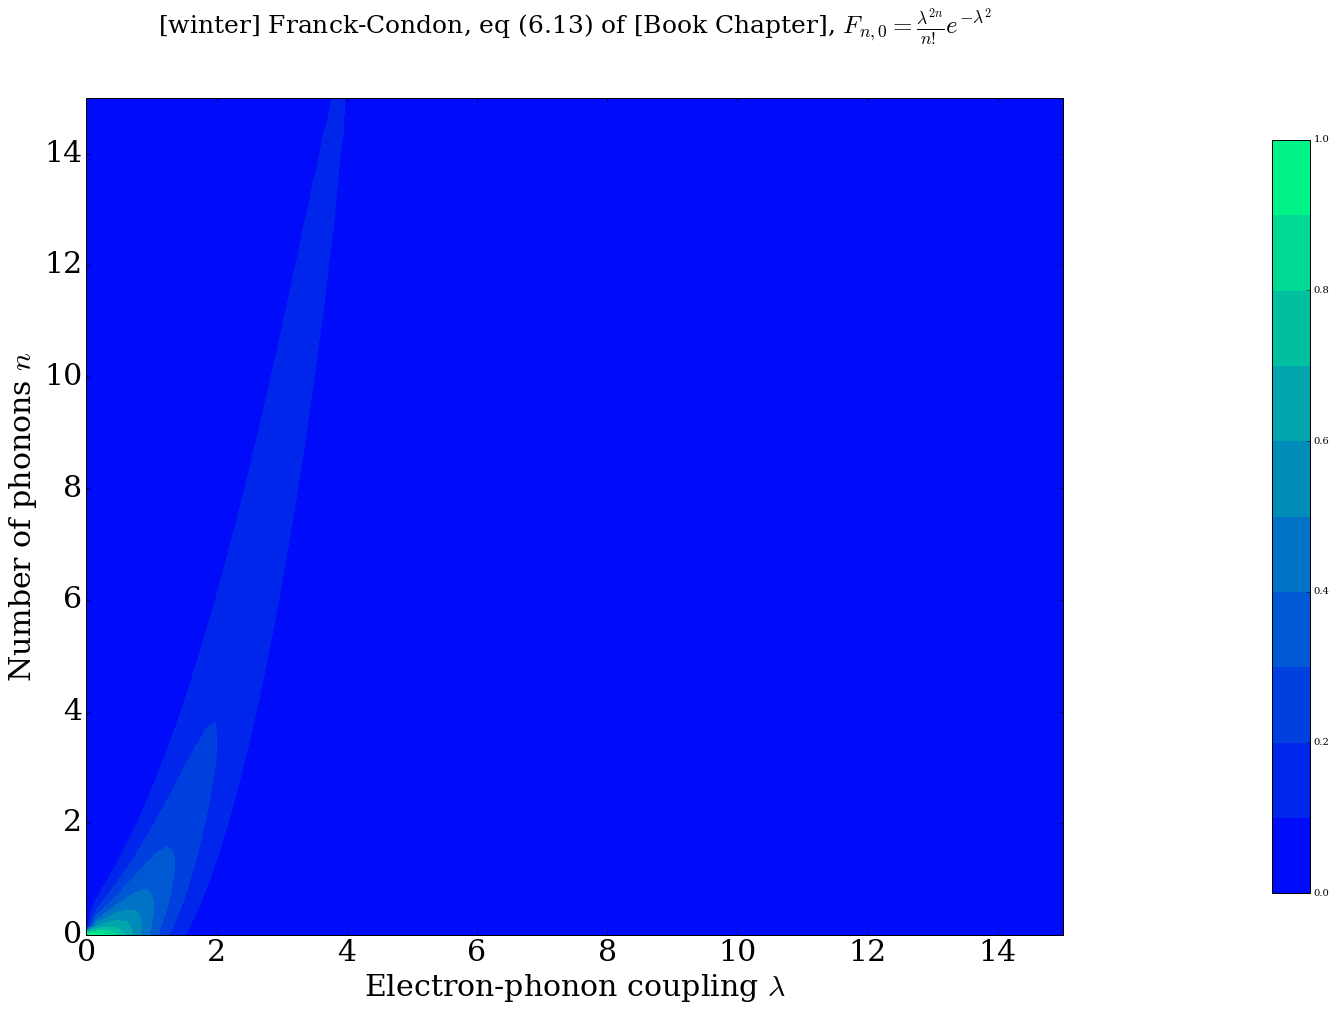
\includegraphics[height=.3\textheight]{png/fcfig.png}
    \caption{Filled contour plot of the ground-to-excited state Franck Condon factors for low coupling. The horizontal-axis describes the coupling strength, whereas the vertical axis denotes the phononic excitation with \emph{number} photons.}
    \label{fig:fc}
\end{figure}

In figure~\ref{fig:fc}, I show the FC-factors for weak electron-phonon coupling. There are three distinct regions. In the $\lambda\ll 1$ region, the only accessible states appear to be those without phonons. As you move closer to unity, exited states become available. Moving away from unity, the zero-excited transition is suppressed, a phenomenon known as the Franck-Condon blockade \cite{fcblockade}.

A typical way in which one confirms the presence of phononic excitations is lines running parallel to the diamond edges in the stability diagram, which is a filled contour plot of the conductance as a function of bias and gate voltage \cite{vibrationcomputation}.

I have already found that the many-body Green's function can be most simply derived as the expectation value of the Green's function operator that includes a complex many-body self-energy operator. I must emphasise that we are working on an extended Hilbert space that does not only include the Hilbert space of electrons $H_e$ but also that of the single-mode vibrations $H_b$. This simplification allows a relatively simple derivation of the many-body Green's function that clearly shows Franck-Condon blockade and vibrational excitations.  

It is worth emphasising that the overlap matrix is not diagonal, because the equilibrium geometry of the molecule changes when the electronic state switches. In a more pedestrian explanation, I would point to classical mechanics. Consider for a moment a very large metal ruler extended over the edge of a desk. On it, I attach a heavy magnet that can't suddenly fly off the ruler. The ruler would act as a cantilever, vibrating in a specific mode. If I suddenly (instantaneously) move the magnet, the mass distribution of  the magnet-ruler system changes, and thus its eigenmodes do as well. However, the ruler is still vibrating in the old mode, which is no longer an eigenmode of the system but rather a superposition of the new eigenmodes, i.e. $\ket{x_j} \rightarrow \sum c_i \ket{x'_i}$. Therefore, the old eigenmode and the new eigenmode are not necessarily orthogonal but have an overlap element. 

I want to use the EOM method to find the self-energy operator. First, it is clear that the commutator between $d_l$ and the Fr\"ohlich interaction is:
\begin{align*}
 \left[ d_l, (b^\dagger + b) d_i^\dagger d_j \right] &= (b^\dagger + b) d_l \delta^j_l
\end{align*}

So that the equation of motion method for the (many-body) Green's function yields:
\begin{align*}
\left(\epsilon-\epsilon_i - \lambda \hbar \omega \left(b^\dagger + b\right) \right) G^\pm (\epsilon) &= \delta_{ij} + \sum_k \left\{ \tau_{ik} + \sum_l U^l_{ik} n_l + \Sigma^\pm_{ik} \right\} G^\pm_{kj}
\end{align*}

And comparison with the Dyson equation results in the self-energy operator for the electron-phonon interaction \footnote{Formally, the term is a constant times the Green's function, so that we multiply it by the unit operator, resulting in a diagonal contribution.}:
\begin{align*}
\Sigma_\text{e-p} &= \lambda \hbar \omega ( b^\dagger + b)
\end{align*}

Recall that, in our previous treatment of the many-body Green's function, we had identified that:
\begin{align*}
\mathscr{G}^{\kappa\pm} \ket{\lambda} &= G^\lambda \Delta^\lambda_\kappa \ket{\lambda}
\end{align*}

Also, we know that operators that act purely on fermions and operators that act purely on bosons commute. This is very convenient because we can now consider a many-body Green's function of a molecule coupled to a single vibrational level, i.e. $\left\{\ket{\kappa}\right\} $ $\rightarrow$ $ \left\{\ket{\kappa}\right\} \otimes \left\{\ket{m}\right\}$, where $\ket{m}$ denotes a vibrational mode.
\begin{align*}
\braket{\mathscr{G}^{\kappa\pm}} &\equiv \sum_{\lambda, \lambda^\prime} \sum_{m,n} \bra{\lambda}\bra{n} \mathscr{G}^{\kappa\pm} \ket{\lambda^\prime}\ket{m} 
\end{align*}

For brevity I define:
\begin{align*}
A &=\left[ \epsilon \mathbf{1} - \mathbf{\epsilon} - \mathbf{\Sigma}^{d\pm} - \mathbf{\Sigma}^\pm \right]^{-1} n_\kappa \\
B &= \Sigma^\pm_\text{e-p}
\end{align*}

Note that $A$ is an operator that only acts on fermionic space, whereas $B$ is an operator that acts on the phonon space. 

I will use the Taylor expansion (equation~\ref{eq:inversionexpansion}), because I will be able to separate terms\footnote{I introduce $\tilde{\lambda}$ for the electron-phonon coupling constant, as our treatment of the many-body Green's function already included the state $\ket{\lambda}$.} because $A$ and $B$ commute:
\begin{align*}
\braket{\mathscr{G}^{\kappa\pm}} &\equiv \sum_{\lambda, \lambda^\prime} \sum_{m,n} \bra{\lambda}\bra{n} \mathscr{G}^{\kappa\pm} \ket{\lambda^\prime}\ket{m} \\
&= \sum_{\lambda, \lambda^\prime} \sum_{m,n}\rho_{\lambda\lambda^\prime}^{mn} \bra{\lambda}\bra{n}\left[A + ABA + ABABA + ABABABA + \ldots\right] \ket{\lambda^\prime}\ket{m} \\
&= \sum_{\lambda, \lambda^\prime} \sum_{m,n} \sum_x\rho_{\lambda\lambda^\prime}^{mn} \braket{\lambda \left| A^{x+1} \right| \lambda^\prime} \braket{n\left| B^x \right|m} \\
&= \sum_{\lambda, \lambda^\prime} \sum_{m,n} \sum_x\rho_{\lambda\lambda^\prime}^{mn} \braket{\lambda \left| A^{x+1} \right| \lambda^\prime} \braket{n\left| \left(\tilde{\lambda}\hbar\omega\right)^x\left(b^\dagger+b\right)^x \right|m} \\ 
\end{align*}

I cannot use Newton's binomial expansion because $b$ and $b^\dagger$ do not commute. However, it is possible to derive the binomial theorem for non-commuting objects, where $\left[A,B\right] = C$. This derivation depends on the dual of the Baker-Campbell-Hausdorff formula \cite{kaspermothpoulsen}, called the Zassenhaus formula \footnote{See e.g. \href{http://goo.gl/Cw8Xpx}{math overflow, http://goo.gl/Cw8Xpx}.}, and takes the general form:
\begin{align*}
(A+B)^n &= \sum_{n\equiv k\:\text{mod}(2)}\left[ \sum^k_{r=0}\left[ \binom{k}{r}A^r B^{k-r} \left(-\frac{C}{2}\right)^\frac{n-k}{2} \frac{n!}{k! \left(\frac{n-k}{2}\right)!}\right]\right] 
\end{align*}
Where $n\equiv k\:\text{mod}(2)$ means that $0\leq k\leq$, but $k$ only takes values that are even (odd) if $n$ is even (odd), so that $\frac{n-k}{2}$ is integer.

By applying this formula, I find:
\begin{align*}
\braket{n \left| \left(b+b^\dagger\right)^x \right| m}&= \sum_{y=x[2]}^x Q^x_y \sum_{p=0}^{y} P^{m,n}_{p,y} \braket{\left. n-p \right| m-y+p}, \\
Q^x_y&\equiv \left(-\frac{1}{2}\right)^{\frac{x-y}{2}} \frac{ x! }{ y! \left(\frac{x-y}{2}\right)!},\\
P_{p,y}^{m,n} &\equiv \binom{y}{p} \sqrt{ \binom{n}{p}} \sqrt{\binom{m}{y-p}}
\end{align*}

For the result above, I have adapted a trick. First, note that $b^n \ket{m} = \binom{m}{n} \ket{m-n}$. Note also that this requires $m\geq n$ to be nonzero. Furthermore, the Hermitian conjugate gives the relation for $\bra{m} (b^\dagger)^n$. As a result, we absorb the creation (annihilation) operators into terms that also put an upper bind on the powers involved. We can freely do so, because the expansion for non-commuting operators remains symmetric; the commutators are in $Q^x_y$. 


The overlap function can be found from the recursion relation, see Ref. \cite{kaspermothpoulsen}:
\begin{align*}
\braket{n|m} &= e^{-\frac{\tilde{\lambda}^2}{2}} \sqrt{n! m!} \sum_{k=0}^{ \text{min}\left\{ m, n \right\}} \frac{ \left(-\tilde{\lambda}\right)^{n-k} \left(\tilde{\lambda}\right)^{m-k}}{ k! \left( n -k\right)! \left( m - k \right)!},
\end{align*} 
where $\tilde{\lambda}$ is the electron-phonon coupling.

This means that we have found a closed form of the vibrational many-body Green's function $\mathscr{G}^{\kappa\pm}_\text{vibrational}$, where the subscript merely denotes that this is on the space $\left\{\ket{\kappa}\right\} \otimes \left\{\ket{n}\right\}$:
\begin{align}
\braket{\mathscr{G}^{\kappa\pm}_\text{vibrational}}&= \sum_{\lambda\supseteq \kappa} \sum_{m,n} \sum_x\rho_{\lambda\lambda^\prime}^{mn}  \left(G^\lambda \right)^{x+1} \left(\tilde{\lambda}\hbar\omega\right)^x
 \sum_{y=x[2]}^x Q^x_y \sum_{p=0}^{y} P^{m,n}_{p,y} \braket{\left. n-p \right| m-y+p} \label{eq:vibgf}
\end{align}

\section{Discussion of Vibrational Interaction}
\label{sec:phononicdiscussion}

Note again that the Taylor expansion is effectively the diagrammatic expansion we also used to derive the Dyson equation. This is a very telling result, because it gives an explanation for the result.

Contrary to fermionic operators, powers of bosonic operators do lead to high multiplicity of specific terms. Although this seems to implicate that the high-order terms cannot be simply assumed to vanish, we must turn to the recursion relation that defines the overlap to investigate this further:
\begin{align*}
\braket{\left. n\right|m} &\equiv \sqrt{\frac{n}{m}} \braket{\left. n-1\right|m-1} + \frac{\lambda}{\sqrt{m}} \braket{\left. n\right|m-1}
\end{align*}

First, note that the overlap goes to zero as $m\gg 1$ due to the inverse proportionality to $\sqrt{m}$. The first term will remain valid in that limit, but only for $n\approx m$, indicating that only few-phonon transitions are possible. If this is combined with the multiplicity of high-order diagrams, this expresses the well-known problem that Feynman diagrammatic expansions are not guaranteed to have vanishing high-order terms \cite{mattuck}.

I think it hopeful that there are various exponentially decaying terms in the full expansion. Combined with the possibility of high-order terms hitting vacuum, I think it is reasonably certain that the near-diagonal high-order terms will be cancelled by these decaying terms. However, that puts a requirement of $ \lambda \hbar \omega < 1$. Given the typical excitation energies of $~100$ meV, this allows for electron-phonon coupling up to $3-5$, which seems sufficient in the low temperature limit. In the ground-state Franck-Condon filled contour (Fig.~\ref{fig:fc}), we saw that this includes most of the relevant part of the picture.

I also think that the expectation value helps to filter high-order contributions, simply because either $n-p$ or $m-y+p$ will hit zero, meaning that all possible phonons are released and higher terms are not possible. 

Let us consider, for a moment, a situation where we assume only a single vibrational mode, and only transitions from the vibrational vacuum to the first few excitations, are relevant. This implies very weak coupling, so assume $\hbar \omega \lambda \approx 0.1$, implying that $x>2$ vanishes. I also assume for the purpose of this example that $\rho^{m,n}_{\lambda\lambda} \approx \rho_{\lambda\lambda} \rho^v_{m,n}$. We would be looking at a term:
\begin{align*}
\mathscr{G}^{\kappa\pm}_\text{vibrational} &= \sum_{\lambda\supseteq \kappa} \rho_{\lambda \lambda} \left[ G^{\lambda\pm} \left( \rho_{00}^v \braket{0|0} + \rho_{10}^v \braket{1|0} + \rho_{20}^v\braket{2|0}\right) \right. \\ &\left.+ \left(\lambda\hbar\omega\right)\left(G^{\lambda\pm}\right)^2 \left(\rho_{10}^v \braket{1|0}\right) + \left(\lambda\hbar\omega\right)^2 \left(G^{\lambda\pm}\right)^3 \left( \rho_{20}^v \braket{0|0}\right) \right]
\end{align*}

Looking back at figure~\ref{fig:fc}, we see clearly that this small expansion should display Franck-Condon blockade quite clearly. Suppose, for instance, that the electron-phonon coupling is very weak. In that case, only $\braket{0|0}$ are significant and we see that the expansion reduces to equation~\ref{eq:mbgfresult}. On the other hand, in the Franck-Condon blockade region, we find only a contribution from $\rho^v_{20} \braket{2|0}$, should be significantly smaller because of the 2 phonon density matrix in that expression.

I have not pursued this derivation further due to time constraints. However, I strongly suggest that it is taken up for further investigation.



%clearpage dumps all images in the stack. Also prevents images from skipping chapters.
\clearpage
\references{dissertation}